\documentclass[a4paper]{article}

% Этот шаблон документа разработан в 2014 году
% Данилом Фёдоровых (danil@fedorovykh.ru) 
% для использования в курсе 
% <<Документы и презентации в \LaTeX>>, записанном НИУ ВШЭ
% для Coursera.org: http://coursera.org/course/latex .
% Исходная версия шаблона --- 
% https://www.writelatex.com/coursera/latex/5.3

% В этом документе преамбула

\usepackage{siunitx}
%%% Работа с русским языком
\usepackage{cmap}					% поиск в PDF
\usepackage{mathtext} 				% русские буквы в формулах
\usepackage[T2A]{fontenc}			% кодировка
\usepackage[utf8]{inputenc}			% кодировка исходного текста
\usepackage[english,russian]{babel}	% локализация и переносы
\usepackage{indentfirst}
\frenchspacing

\renewcommand{\epsilon}{\ensuremath{\varepsilon}}
\renewcommand{\phi}{\ensuremath{\varphi}}
\renewcommand{\kappa}{\ensuremath{\varkappa}}
\renewcommand{\le}{\ensuremath{\leqslant}}
\renewcommand{\leq}{\ensuremath{\leqslant}}
\renewcommand{\ge}{\ensuremath{\geqslant}}
\renewcommand{\geq}{\ensuremath{\geqslant}}
\renewcommand{\emptyset}{\varnothing}
\renewcommand{\Im}{\operatorname{Im}}
\renewcommand{\Re}{\operatorname{Re}}


%%% Дополнительная работа с математикой
\usepackage{amsmath,amsfonts,amssymb,amsthm,mathtools} % AMS
\usepackage{icomma} % "Умная" запятая: $0,2$ --- число, $0, 2$ --- перечисление

%% Номера формул
%\mathtoolsset{showonlyrefs=true} % Показывать номера только у тех формул, на которые есть \eqref{} в тексте.
%\usepackage{leqno} % Нумереация формул слева

%% Свои команды
\DeclareMathOperator{\sgn}{\mathop{sgn}}
\DeclareMathOperator{\sign}{\mathop{sign}}
\DeclareMathOperator*{\res}{\mathop{res}}
\DeclareMathOperator*{\tr}{\mathop{tr}}

%% Перенос знаков в формулах (по Львовскому)
\newcommand*{\hm}[1]{#1\nobreak\discretionary{}
{\hbox{$\mathsurround=0pt #1$}}{}}

%%% Работа с картинками
\usepackage{graphicx}  % Для вставки рисунков
\graphicspath{{figures/}}  % папки с картинками
\setlength\fboxsep{3pt} % Отступ рамки \fbox{} от рисунка
\setlength\fboxrule{1pt} % Толщина линий рамки \fbox{}
\usepackage{wrapfig} % Обтекание рисунков текстом

%%% Работа с таблицами
\usepackage{array,tabularx,tabulary,booktabs} % Дополнительная работа с таблицами
\usepackage{longtable}  % Длинные таблицы
\usepackage{multirow} % Слияние строк в таблице

%%% Теоремы
\theoremstyle{plain} % Это стиль по умолчанию, его можно не переопределять.
\newtheorem{theorem}{Теорема}
\newtheorem*{thm}{Теорема}
\newtheorem{prop}{Утверждение}
 
\theoremstyle{definition} % "Определение"
%\newtheorem{corollary}{Следствие}[theorem]
\newtheorem*{dfn}{Определение}
\newtheorem{problem}{Задача}
\newtheorem*{problem*}{Задача}

 
\theoremstyle{remark} % "Примечание"
\newtheorem*{sol}{Решение}
\newtheorem*{rem}{Замечание}

%%% Программирование
\usepackage{etoolbox} % логические операторы

%%% Страница
%\usepackage{extsizes} % Возможность сделать 14-й шрифт
%\usepackage{geometry} % Простой способ задавать поля
%	\geometry{top=25mm}
%	\geometry{bottom=35mm}
%	\geometry{left=35mm}
%	\geometry{right=20mm}
 
\usepackage{fancyhdr} % Колонтитулы
%	\pagestyle{fancy}
 %	\renewcommand{\headrulewidth}{0pt}  % Толщина линейки, отчеркивающей верхний колонтитул
	%\lfoot{Нижний левый}
	%\rfoot{Нижний правый}
	%\rhead{Верхний правый}
	%\chead{Верхний в центре}
	%\lhead{Верхний левый}
	%\cfoot{Нижний в центре} % По умолчанию здесь номер страницы

\usepackage{setspace} % Интерлиньяж
%\onehalfspacing % Интерлиньяж 1.5
%\doublespacing % Интерлиньяж 2
%\singlespacing % Интерлиньяж 1

\usepackage{lastpage} % Узнать, сколько всего страниц в документе.

\usepackage{soul} % Модификаторы начертания

\usepackage{hyperref}
%\usepackage[usenames,dvipsnames,svgnames,table,rgb]{xcolor}
\hypersetup{				% Гиперссылки
    unicode=true,           % русские буквы в раздела PDF
    pdftitle={Заголовок},   % Заголовок
    pdfauthor={Автор},      % Автор
    pdfsubject={Тема},      % Тема
    pdfcreator={Создатель}, % Создатель
    pdfproducer={Производитель}, % Производитель
    pdfkeywords={keyword1} {key2} {key3}, % Ключевые слова
    colorlinks=true,       	% false: ссылки в рамках; true: цветные ссылки
    linkcolor=red,          % внутренние ссылки
    citecolor=black,        % на библиографию
    filecolor=magenta,      % на файлы
    urlcolor=cyan           % на URL
}

\usepackage{csquotes} % Еще инструменты для ссылок

%\usepackage[style=apa,maxcitenames=2,backend=biber,sorting=nty]{biblatex}

\usepackage{multicol} % Несколько колонок

\usepackage{tikz} % Работа с графикой
\usepackage{pgfplots}
\usepackage{pgfplotstable}
%\usepackage{coloremoji}
\usepackage{floatrow}
\usepackage{subcaption}
\newcommand*{\N}{\mathbb{N}}
\newcommand*{\R}{\mathbb{R}}
\newcommand*{\K}{\mathbb{K}}
\newcommand*{\V}{\mathcal{V}}
\newcommand*{\A}{\mathcal{A}}
\newcommand*{\ii}{\mathbf{1}}
\newcommand*{\oo}{\mathbf{0}}
\newcommand*{\ba}{\mathbf{a}}
\newcommand*{\bb}{\mathbf{b}}
\newcommand*{\Q}{\mathbb{Q}}
\graphicspath{{figures/}}
%\usepackage{breqn}

\renewcommand\thesubfigure{\asbuk{subfigure}}
%\addbibresource{master.bib}

\usepackage{import}
\usepackage{pdfpages}
\usepackage{transparent}
\usepackage{xcolor}
\usepackage{xifthen}

%\newcommand{\incfig}[1]{%
%    \def\svgwidth{\columnwidth}
%    \import{./figures/}{#1.pdf_tex}
%}


\newcommand{\incfig}[2][1]{%
    \def\svgwidth{#1\columnwidth}
    \import{./figures/}{#2.pdf_tex}
}
\usepackage{titlesec}
%\titleformat{\section}{\normalfont\Large\bfseries}{}{0pt}{}
%----------------------STANDART:
%\titleformat{\chapter}[display]
%  {\normalfont\huge\bfseries}{\chaptertitlename\ \thechapter}{20pt}{\Huge}
%\titleformat{\section}{\normalfont\Large\bfseries}{\thesection}{1em}{}
%\titleformat{\subsection}
%  {\normalfont\large\bfseries}{\thesubsection}{1em}{}
%\titleformat{\subsubsection}
%  {\normalfont\normalsize\bfseries}{\thesubsubsection}{1em}{}
%\titleformat{\paragraph}[runin]
%  {\normalfont\normalsize\bfseries}{\theparagraph}{1em}{}
%\titleformat{\subparagraph}[runin]
%  {\normalfont\normalsize\bfseries}{\thesubparagraph}{1em}{}

\pdfsuppresswarningpagegroup=1
\pgfplotsset{compat=1.16}

\usepackage{xifthen}
\makeatother
%\def\@lecture{}%
%\newcommand{\lecture}[3]{
%    \ifthenelse{\isempty{#3}}{%
%        \def\@lecture{Неделя #1}%
%    }{%
%        \def\@lecture{Неделя #1: #3}%
%    }%
%    \section*{\@lecture}
%    \marginpar{\small\textsf{\mbox{#2}}}
%}
\makeatletter

%\newcommand{\lec}{\subsection{Лекция}}
%\newcommand{\sem}{\subsection{Семинар}}
%\newcommand{\hw}{\subsection{Домашняя работа}}
%\newcommand{\prob}[1]{\textbf{#1}}
%\renewcommand{\thesubsection}{}
%\renewcommand{\thesubsubsection}{}

%\setcounter{tocdepth}{1} % only parts,chapters,sections
%\titleformat{\subsection}{\normalfont\large\bfseries}{}{0em}{}
%\titleformat{\subsubsection}{\normalfont\normalsize\bfseries}{}{0em}{}

%\newcommand{\textover}[2]{\stackrel{\mathclap{\normalfont\mbox{#2}}}{#1}}

\author{Драчов Ярослав\\
Факультет общей и прикладной физики МФТИ}
\newcommand{\veq}{\mathrel{\rotatebox{90}{$=$}}}
%\newcommand{\teto}[1]{\stackrel{\mathclap{\normalfont\tiny\mbox{#1}}}{\to}}
%\renewcommand{\thesubsection}{\arabic{subsection}}

%%\setcounter{secnumdepth}{0}

\definecolor{tabblue}{RGB}{30, 119, 180}
\definecolor{taborange}{RGB}{255, 127, 15}
\definecolor{tabgreen}{RGB}{45, 160, 43}
\definecolor{tabred}{RGB}{214, 38, 40}
\definecolor{tabpurple}{RGB}{148, 103, 189}
\definecolor{tabbrown}{RGB}{140, 86, 76}
\definecolor{tabpink}{RGB}{227, 119, 193}
\definecolor{tabgray}{RGB}{127, 127, 127}
\definecolor{tabolive}{RGB}{188, 189, 33}
\definecolor{tabcyan}{RGB}{22, 190, 207}
\pgfplotscreateplotcyclelist{colorbrewer-tab}{
{tabblue},
{taborange},
{tabgreen},
{tabred},
{tabpurple},
{tabbrown},
{tabpink},
{tabgray},
{tabolive},
{tabcyan},
}
\usepackage{csvsimple}
\usepackage{extarrows}
%\renewcommand{\labelenumii}{\asbuk{enumii})}
%\renewcommand{\labelenumiv}{\Asbuk{enumiv}}
\newcommand{\prob}[1]{\subsubsection*{#1}}
\sisetup{output-decimal-marker = {,},separate-uncertainty = true,exponent-product = \cdot}

\usepackage{braket}
\usepackage{enumerate}
\usepackage{chngcntr}
%\counterwithin*{equation}{problem}
%\usepackage{bbold}

\newtheoremstyle{hiProb}% ⟨name ⟩ 
{3pt}% ⟨Space above ⟩1 
{3pt}% ⟨Space below ⟩1
{}% ⟨Body font ⟩
{}% ⟨Indent amount ⟩2
{\bfseries}% ⟨Theorem head font⟩
{.}% ⟨Punctuation after theorem head ⟩
{.5em}% ⟨Space after theorem head ⟩3
%{\thmname{#1} \thmnote{#3}}% ⟨Theorem head spec (can be left empty, meaning ‘normal’)⟩
{\thmnote{#3}}% ⟨Theorem head spec (can be left empty, meaning ‘normal’)⟩
\theoremstyle{hiProb} % "Определение"
%\newtheorem{hiProb}{Задача}
\newtheorem{hiProb}{}
\usepackage{mmacells}
\newcommand{\textover}[2]{\stackrel{\mathclap{\normalfont\scriptsize\mbox{#2}}}{#1}}
\usepackage{units}
\usepackage[math]{cellspace}%
\setlength\cellspacetoplimit{2pt}
\setlength\cellspacebottomlimit{2pt}

\usepackage[backend=biber,bibencoding=utf8,sorting=ynt,maxcitenames=2,style=numeric]{biblatex}
\addbibresource{bib.bib}
\title{Лабораторная работа №2.1\\  <<Опыт Франка-Герца>>}
\author{Драчов Ярослав \\ Факультет общей и прикладной физики МФТИ}
\begin{document}
\maketitle
\begin{abstract}
	В данной работе методом электронного возбуждения будет
	измерена энергия первого уровня атома гелия в динамическом
	и статическом режимах.
\end{abstract}
\section{Теоретическое введение}
Одним из простых опытов, подтверждающих существование дискретных
уровней энергии атомоов, является эксперимент, известный под
названием опыта Франка и Герца. Схема опыта изображена на рис.~\ref{fig:1}
\begin{figure}[ht]
	\centering
	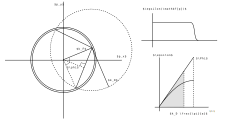
\includegraphics[width=0.6\textwidth]{1}
	\caption{Принципиальная схема опыта Франка и Герца}
	\label{fig:1}
\end{figure}

Разреженный одноатомный газ (в нашем случае --- гелий) заполняет
трёхэлектродную лампу. Электроны, испускаемые разогретым
катодом, ускоряются в постоянном электрическом поле, созданным
между катодом и сетчатым анодом лампы. Передвигаясь от катода
к аноду, электроны сталкиваются с атомами гелия. Если энергия
электрона, налетающего на атом, недостаточна для того, чтобы
перевести его в возбуждённое состояние (или ионизовать), то
возможны только упругие соударения, при которых электроны
почти не теряют энергии, так как их масса в тысячи раз меньше
массы атомов.

По мере увеличения разности потенциалов между анодом и катодом
энергия электронов увеличивается и, в конце концов, оказывается
достаточной для возбуждения атомов. При таких --- неупругих ---
столкновениях кинетическая энергия налетающегоо электрона
передаётся одному из атомных электронов, вызывая его переход
на свободный энергетический уровень (возбуждение) или
совсем отрывая его от атома (ионизация).

Третьим электродом лампы является коллектор. Между ним и анодом
поддерживается небольшое задерживающее напряжении (потенциал
коллектора меньше потенциала анода). Ток коллектора, пропорциональный
числу попадающих на него за секунду электронов, измеряется
микроамперметром.

При увеличении потенциала анода ток в лампе вначале
растёт, подобно тому как это происходит в вакуумном диоде (рис.~\ref{fig:2}).
\begin{figure}[ht]
	\centering
	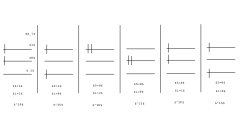
\includegraphics[width=0.4\textwidth]{2}
	\caption{Зависимость тока коллектора от напряжения на аноде}
	\label{fig:2}
\end{figure}Однако, когда энергия электронов становится достаточной
 для возбуждения атомов, ток коллектора резко уменьшается. Это
происходит  потому, что при неупругих соударениях с атомами электроны
почти полностью теряют свою энергию и не могут преодолеть
задерживающего потенциала (около 1 В) между анодом и коллектором.
При дальнейшем увеличении потенциала анода ток коллектора
вновь воозрастает: электроны, испытавшие неупругие соударения, при
дальнейшем движении к аноду
успевают набрать энергию, достаточную для преодоления задерживающего
потенциала.

Следующее замедление роста тока происходит в момент, когда часть
электронорв неупруго сталкиваетсяя с атомами два раза: первый
раз посередине пути, второй --- у анода, и т.д. Таким образом, на
кривой зависимости тока коллектора от напряжения анода имеется
ряд максимумов и минимумов, отстоящих друг от друга на равные
расстояния $\Delta V$; эти расстояния равны энергии первого
возбуждённого состояния (рис.~\ref{fig:2}).

При тщательной постановке опыта можно увидеть и тонкую структуру
кривой спада тока, содержащую ряд минимумов, соответствующих
возбуждению других уровней и ионизации атома гелия. Для этого
нужны лампы специальной конструкции. В нашей постановке опыта
эта тонкая структура не видна.

\section{Экспериментальная установка}
Схема экспериментальной установки изображена на рис.~\ref{fig:3}.
\begin{figure}[ht]
	\centering
	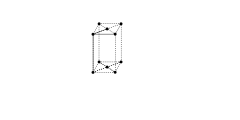
\includegraphics[width=0.6\textwidth]{3}
	\caption{Схема экспериментальной установки}
	\label{fig:3}
\end{figure}
Для опыта используется серийная лампа ионизационнго манометра ЛМ-2,
заполненная гелием до давления $\sim 1$ Торр. Источником электронов
является вольфрамовый катод, нагреваемый переменным током. Наряжение
накала подаётся от стабилизируемого источника питания С. Ток
накала контролируется амперметром А.

В качестве анода используется двойная спираль, окружающая катод.
Роль коллектора играет полый металлический цилиндр, соосный с катодом
и анодом.

Ускоряющее напряжение подаётся на анод от выпрямителя В. Величина
этого напряжения регулируется потенциометром $\Pi_3$ и измеряется
вольтметром $V_1$. 

Источник задерживающего напряжения --- батарея 4,5 В; величина
напряжения регулируется потенциометром $\Pi_2$ и измеряется
вольтметром $V_2$. Ток в цепи коллектора регистрируется микроамперметром.

Схему меожно переключать из статического режим измерения в
динамический режим с помощью ключа $K_3$. На рис.~\ref{fig:3} две
части сдвоенного ключа $K_3$ изображены отдельно. При динамическом
режиме работы ускоряющий потенциал подаётся с понижающего
трансформатора $T$ (220/50 В), а ток коллектора регистрируется
осциллографом, подключённым к нагрузочному резистору $R$.

При определении энергии электронов по разности потенциалов между
анодом и катодом следует иметь в виду, что из-за контактной
разности потенциалов между катодом и анодом первый максимум не
соответствует потенциалу первого возбуждённого уровня. Однако
контактная разность потенциалов сдвигает все максимумы одинаково,
так что расстояние между ними не меняется.

Схема экспериментальной установки, изображённой на рис.~\ref{fig:3},
 в нашей работе коструктивно осуществлена следующим образом.
Наполненная гелием лампа ЛМ-2 расположена непосредственно на корпусе
блока источников питания (БИП). Напряжение к электродам лампы
подводится от источников питания, находящихся в корпусе прибора.
Регулировка напряжения и выбор режима работы
производятся при помощи ручек управления, выведенных на лицевую
панель БИП (рис.~\ref{fig:4}).
\begin{figure}[ht]
	\centering
	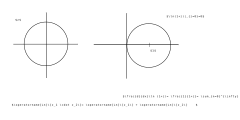
\includegraphics[width=0.8\textwidth]{4}
	\caption{Блок-схема экспериментальной установки}
	\label{fig:4}
\end{figure}
Включении всех источников питания осуществляется
включением БИП в сеть.

В статическом режиме напряжение $V_\text{а}$ между анодом и катодом
измеряется цифровым вольтметром В7-22А, подключённым к клеммам
<<Вольтметр>> прибора. Ток коллектора $I_\text{к}$ измеряется
микроамперметром, вся шкала которого соответствует току 100 мкА.

\section{Ход работы}
Полученные в ходе измерений зависимости представлены в таблице~\ref{tab:1}.

\begin{table}[h]
\centering
\begin{subtable}[h]{0.25\textwidth}
\centering
\begin{tabular}{|l|l|}
\hline
$V_{\text{а}} $, В     & $I_{\text{к}}$, дел    \\ \hline
73   & 100 \\ \hline
56   & 90  \\ \hline
49   & 80  \\ \hline
45   & 76  \\ \hline
37   & 81  \\ \hline
32   & 70  \\ \hline
29,3 & 60  \\ \hline
26,1 & 50  \\ \hline
24,7 & 47  \\ \hline
24,3 & 56  \\ \hline
17,5 & 50  \\ \hline
14,3 & 40  \\ \hline
11,0   & 30  \\ \hline
8,2  & 20  \\ \hline
4,7  & 10  \\ \hline
0,0    & 0   \\ \hline
\end{tabular}
\caption{$V_2=4 \text{ В}$ }
\end{subtable}
\hfill
\begin{subtable}[h]{0.25\textwidth}
\centering
\begin{tabular}{|l|l|}
\hline
$V_{\text{а}} $, В     & $I_{\text{к}}$, дел    \\ \hline
74   & 100 \\ \hline
55   & 90  \\ \hline
48   & 81  \\ \hline
38   & 96  \\ \hline
32,6 & 80  \\ \hline
30,9 & 70  \\ \hline
28,9 & 60  \\ \hline
27,3 & 50  \\ \hline
25,4 & 45  \\ \hline
23,6 & 77  \\ \hline
17,3 & 60  \\ \hline
13,0   & 40  \\ \hline
8,57 & 20  \\ \hline
0,00    & 0   \\ \hline
\end{tabular}
\caption{$V_2=6 \text{ В}$ }
\end{subtable}
\hfill
\begin{subtable}[h]{0.25\textwidth}
\centering
\begin{tabular}{|l|l|}
\hline
$V_{\text{а}} $, В     & $I_{\text{к}}$, дел    \\ \hline
74   & 77 \\ \hline
63   & 83 \\ \hline
53   & 70 \\ \hline
50   & 68 \\ \hline
38   & 93 \\ \hline
32,7 & 70 \\ \hline
30,2 & 50 \\ \hline
26,3 & 33 \\ \hline
23,8 & 89 \\ \hline
15,5 & 50 \\ \hline
0,0    & 0  \\ \hline
\end{tabular}
\caption{$V_2=8 \text{ В}$ }
\end{subtable}
\caption{Зависимость коллекторного тока $I_{\text{к}}$ от анодного
	напряжения $V_{\text{а}}$ для 3-х значений задерживающего напряжения
$V_2=4,\,6,\,8 \text{ В}$}
\label{tab:1}
\end{table}
Построим графики $I_{\text{к}}=f(V_{\text{а}})$ для всех значений
$V_2$ (рис.~\ref{fig:hi}).
\begin{figure}
     \centering
     \begin{subfigure}[b]{0.6\textwidth}
         \centering
         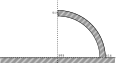
\includegraphics[width=\textwidth]{5}
         \caption{$V_2=4$ В}
         \label{fig:5}
     \end{subfigure}
     \hfill
     \begin{subfigure}[b]{0.6\textwidth}
         \centering
         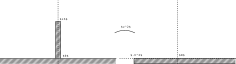
\includegraphics[width=\textwidth]{7}
         \caption{$V_2=6$ В}
         \label{fig:6}
     \end{subfigure}
     \hfill
     \begin{subfigure}[b]{0.6\textwidth}
         \centering
         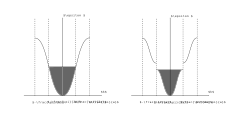
\includegraphics[width=\textwidth]{6}
         \caption{$V_2=8$ В}
         \label{fig:7}
     \end{subfigure}
        \caption{Зависимость коллекторного тока $I_{\text{к}}$ от анодного
	напряжения $V_{\text{а}}$ для 3-х значений задерживающего напряжения
$V_2$}
        \label{fig:hi}
\end{figure}
Для определения энергии первого возбуждённого состояния гелия
найдём расстояния $\Delta V$ между первыми двумя максимами
и минимумами для каждого значения задерживающего напряжения
найдём среднее значение для этих величин:
 \[
V = 17,1\pm 0,4 \text{ В}
.\]
Следовательно, по результатам эксперимента мы получаем, что
энергия первого возбуждённого состояния гелия
\[
W= 17,1\pm 0,4 \text{ эВ}
.\]
По порядку это согласуется с табличным значением (рис.~\ref{fig:8})
\[
W \approx 20,55 \text{ эВ}
.\] 
\section{Выводы}
В данной работе методом электронного возбуждения была
измерена энергия первого уровня атома гелия в динамическом
и статическом режимах, экспериментальные результаты сходятся по
порядку с табличными данными.
\printbibliography
\newpage
\appendix
\section{Приложение}
\begin{figure}[ht]
	\centering
	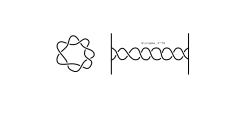
\includegraphics[width=\textwidth]{8}
	\caption{Схемы термов для пара- и ортогелия с одним электроном в основном состоянии $1S$ и одним возбужденным электроном.\cite{wiki:xxx}}
	\label{fig:8}
\end{figure}
\end{document}
